%%%%%%%%%%%%%%%%%%%%%%%%%%%%%%%%%%%%%%%%%%%%%%%%%%%%%%%%%%%%%%%%%%%%%%%%%
% This file is part of the LaTeX sources of the OMDoc 1.3 specification
% Copyright (c) 2016 Michael Kohlhase.
% Source at https://github.com/KWARC/OMDoc/tree/master/doc/spec
% This work is licensed by the Creative Commons Share-Alike license
% see http://creativecommons.org/licenses/by-sa/2.5/ for details
%%%%%%%%%%%%%%%%%%%%%%%%%%%%%%%%%%%%%%%%%%%%%%%%%%%%%%%%%%%%%%%%%%%%%%%%%

\begin{tchapter}[id=markup-web]{Document Markup for the Web}
Document markup is the process of adding codes to a document to identify the
structure of a document and to specify the format in which its fragments are to
appear. We will discuss two conflicting aspects --- structure and appearance ---
in document markup. As the Internet imposes special constraints imposed on markup
formats, we will reflect its influence.

In the past few years the {\xml} format has established itself as a general basis for
markup languages. As {\omdoc} and all mathematical markup schemes discussed here are
{\xml} applications\twin{XML}{application} (instances of the {\xml}
framework)\twin{XML}{application}, we will go more into the technical details to supply
the technical prerequisites for understanding the specification.  We will briefly mention
{\xml} validation and transformation tools, if the material reviewed in this section is
not enough, we refer the reader to~\cite{Harold:xb01}.

\begin{tsection}[id=markup-types]{Structure vs. Appearance in Markup}

  Text processors and desktop publishing systems (think for example of
  {\twintoo{Microsoft}{Word}}) are software systems aiming to produce
  ``{\emin{ink-on-paper}}'' or ``{\emin{pixel-on-screen}}'' representations of documents.
  They are very well-suited to execute typographic conventions for the appearance of
  documents. Their internal markup scheme mainly defines presentation traits like
  character position, font choice and characteristics, or page breaks.  We will speak of
  {\twindef{presentation}{markup}} for such markup schemes.  They are perfectly sufficient
  for producing high-quality presentations on paper or on screen, but for instance it does
  not support document reuse (in other contexts or across the development cycle of a
  text). The problem is that these approaches concentrate on the {\emin{form}} and not the
  {\emin{function}} of text elements.  Think e.g. of the notorious section renumbering
  problems in early ({\indextoo{WYSIWYG}}\footnote{``What you see is what you get''; in
    the context of markup languages this means that the document markup codes are hidden
    from the user, who is presented with a presentation form of the text even during
    authoring.}) text processors.  Here, the text form of a numbered section heading was
  used to express the function of identifying the position of the respective section in a
  sequence of sections (and maybe in a larger structure like a chapter).

  This perceived weakness has lead to markup schemes that concentrate more on function
  than on form.  We will call them {\twindef{content}{markup}} to distinguish them from
  presentation markup schemes, and discuss {\index{latex@\LaTeX}\index{tex@\TeX}}
  {\TeX}/{\LaTeX} {\cite{Knuth:ttb84,Lamport:ladps94}} as an example.

  {\TeX} is a typesetting markup language that uses explicit markup codes (strings
  beginning with a backslash) in a document, for instance, the markup
  {\verb|$\sqrt{\sin x}$|} stands for the mathematical expression $\sqrt{\sin x}$ in
  {\TeX}. To determine from this functional specification the visual form (e.g. the
  character placement and font information), we need a document formatting engine.  This
  program will transform the document that contains the content markup (the
  ``{\indextoo{source}}'' document\twin{document}{source}) into a presentation markup
  scheme that specifies the appearance (the ``{\indextoo{target}}''
  document\twin{document}{target}) like {DVI\index{dvi@DVI}}~\cite{Knuth:ttb84},
  {\sc{post\-script}}~\cite{Reid:plpd87}, or {\scsys{PDF}}~\cite{PDFReference} that can
  directly be presented on paper or on screen.  This two-stage approach allows the author
  to mark up the function of a text fragment and leave the conversion of this markup into
  presentation information to the formatter. The specific form of translation is either
  hard-wired into the formatter, or given externally in {\emph{\twintoo{style}{file}s}} or
  {\emph{\indextoo{style sheet}s}}.

{\LaTeX}~\cite{Lamport:ladps94}\twin{style}{file} is a comprehensive set of style
files for the {\TeX} formatter, the heading for a section with the title ``The Joy
of {\TeX}'' would be marked up as
\begin{small}
\begin{verbatim}
\section[{\TeX}]{The Joy of {\TeX}\index{tex@\TeX}}\label{sec:TeX}
\end{verbatim}
\end{small}
This piece of markup specifies the function of the text element: The title of the section
should be ``The Joy of {\TeX}'', which (if needed e.g. in the table of contents) can be
abbreviated as ``{\TeX}'', the glyph ``{\TeX}'' is inserted into the index, where the word
{\tt{tex}} would have been, and the section number can be referred to using the label
{\snippet{sec:TeX}}.  Note that {\indextoo{renumbering}} is not a problem in this
approach, since the actual numbers are only inferred by the formatter at run-time. This,
together with the ability to simply change style file for a different context, yields much
more manageable and reusable documents, and has led to a wide adoption of the
function-based approach. So that even word-processors like MS Word now include functional
elements. Pure presentation markup schemes like {DVI\index{dvi@DVI}} or {\postscript} are
normally only used for document delivery. On the other hand, many form-oriented markup
schemes allow to ``fine-tune'' documents by directly controlling presentation. For
instance, {\LaTeX} allows to specify traits such as font size information, or using
\begin{center}
  {\verb+{\bf proof}:+}\ldots{\verb+\hfill\Box+}
\end{center}
to indicate the extent of a proof (the formatter only needs to ``copy'' them to
the target format). The general experience in such mixed markup schemes is that
presentation markup is more easily specified, but that content markup will enhance
maintainability and reusability. This has led to a culture of style file
development (specifying typographical and structural conventions), which now gives
us a wealth of style options to choose from in {\LaTeX}.
\end{tsection}

\begin{tsection}[id=markup:www]{Markup for the World Wide Web}{}

The Internet, where screen presentation, hyperlinking, computational limitations,
and bandwidth considerations are much more important than in the ``ink-on-paper''
world of publishing, has brought about a whole new set of markup schemes. The
problems that need to be addressed are that
\begin{itemize}
\item the size, resolution, and color depth of a given screen are not known at the time
  the document is marked up,
\item the structure of a text is no longer limited to a linear text with (e.g.  numbered)
  {\indextoo{cross-reference}s} as in a traditional book or article: Internet documents
  are usually hypertexts,
\item the computational resources of the computer driving the screen are not known
  beforehand. Therefore the distribution of work (e.g. formatting steps) between the
  client and the server has to be determined at run-time. Finally, the related problem that
\item the bandwidth of the Internet is ever-growing but always limited.
\end{itemize}

These issues impose somewhat conflicting demands on markup languages for the Web.  The
first two seem to favor content markup languages, since low-level presentational traits
like glyph placement and font availability cannot be pre-meditated on the server. However,
the amount of formatting that can be delegated to the client, and the availability of
style files is limited by the latter two concerns.

In response the ``{\indextoo{Hypertext Markup Language}}'' ({\html}~\cite{RagHor:html98})
evolved as the original markup format for the {\twintoo{World Wide}{Web}}. This is a
markup scheme that addresses the problem of variable screen size and hyperlinking by
exporting the decision of character placement and page order to a {\indextoo{browser}}
running on the client.  It ensures a high degree of reusability of documents on the
Internet while conserving bandwidth, so that {\html} carries most of the text markup on
the Internet today.

The major innovation in {\html} was the use of {\atwindef{uniform}{resource}{locator}s}
({\defin{URL}}) to reference documents provided by web servers. URLs are strings in a
special format that can be interpreted by browsers or other {\twintoo{web}{agent}s} to
request documents from web servers, e.g. to be displayed to the user in the browser as a
new node in the current {\twintoo{hypertext}{document}}. Since URLs are global references,
they are the means that make the Internet into a ``{\em{world-wide}}'' web (of
references).  Since uniform resource {\emph{locators}} are closely tied to the physical
location of a document on the Internet, which can change over time, they have since been
generalized to {\atwindef{uniform}{resource}{identifier}} ({\defin{URI}};
see~\cite{BerFie:uri98}). These are strings of similar structure, that only identify
resources on the Internet, see~\cite{Harold:xb01}, i.e. their structure need not be
directly translatable to an Internet location (we call this act
{\defin{de-referencing}}). Indeed, URIs need not even correspond to a physical
manifestation of a resource at all, they can identify a virtual resource, that is produced
by a web service on demand.

The concrete syntax and architecture of {\html} is derived from the ``{\indextoo{Simple
    Generalized Markup Language}}'' {\sgml}~\cite{Goldfarb:sgml90}, which is similar to
{\TeX/LaTeX} in spirit, but tries to give the markup scheme a more declarative semantics
(as opposed to the purely procedural -- and rather baroque -- semantics of {\TeX}) to make
it simpler to reason about (and thus reuse) documents. In particular unlike {\TeX},
{\sgml} separates content markup codes from directives to the formatting engine.  {\sgml}
has a separate {\indextoo{style sheet}} language\twin{language}{style sheet}
{\dsssl}~\cite{DuCharme:fddsj97}, which was not adopted by {\html}, because of resource
limitations in the client. Instead, {\html} has been augmented with its own (limited)
style sheet language {\css}~\cite{BosHak:css98} that is executed by the browser.
\end{tsection}

\begin{tsection}[id=xml]{XML, the eXtensible Markup Language}

  The need for content markup schemes for maintaining documents on the server, as well as
  for specialized presentation of certain text parts (e.g. for mathematical or chemical
  formulae), has led to a profusion of markup schemes for the Internet, most of which
  share the basic {\sgml} syntax with {\html}.  To organize this zoo of markup languages,
  the {\atwintoo{World Wide}{Web}{Consortium}} ({\indextoo{W3C}}~\cite{W3C:online}, an
  international interest group of universities and web industry) has developed a language
  framework for Internet markup languages called {\xml} (e{\underline{X}}tensible
  {\underline{M}}arkup {\underline{L}}anguage)~\cite{Bray:XML97}. {\xml} is a set of
  grammar rules that allows to interpret certain sequences of
  {\indextoo{Unicode}}~\cite{Unicode:tuc03} characters as document trees. These grammar
  rules are shared by all {\xml}-based markup languages (called {\xml}
  applications\index{application!{\sc Xml}}) and are very well-supported by a great
  variety of {\xml} processors\index{processor!{\sc{Xml}}}. The {\xml} format is
  accompanied by a set of specialized vocabularies (most of them {\xml} applications) that
  standardize various aspects of {\twintoo{document}{management}} and
  {\twintoo{web}{service}s}. These are canonicalized by the W3C as
  ``{\indextoo{recommendation}s}''. We will briefly review the ones that are relevant for
  understanding the {\omdoc} format and make the book self-contained. For details see one
  of the many {\xml} books, e.g.~\cite{Harold:xb01}.

\begin{tsubsection}[id=xml-tree,short=XML Documents as Trees]{XML Document Trees} 
  \begin{myfig}{xml-tree}{An {\xml} Document as a Tree}
    \begin{center}
      \begin{minipage}{9cm}
\begin{lstlisting}[numbers=none]
<omtext xml:id="foo" xmlns="http://omdoc.org/ns"
        xmlns:om="http://www.openmath.org/OpenMath">
  <CMP xml:lang='en'><xhtml:p>
   The number 
   <om:OMOBJ><om:OMS cd="nums1" name="pi"/><om:OMOBJ> 
   is irrational.   
  </xhtml:p></CMP>
</omtext>
\end{lstlisting}
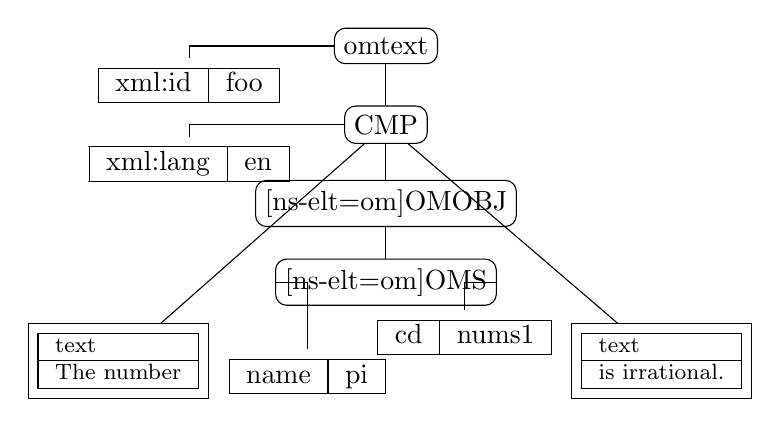
\begin{tikzpicture}
  \node (omtext) [draw,rounded corners] at (2,4) {\element{omtext}};
  \node (CMP) [draw,rounded corners] at (2,3) {\element{CMP}};
  \node (xmlid) at (-.5,3.5) {\begin{tabular}{|c|c|}\hline xml:id& foo \\\hline\end{tabular}};
  \node (xmllang) at (-.5,2.5) {\begin{tabular}{|c|c|}\hline xml:lang& en \\\hline\end{tabular}};
  \node (text1) [draw] at (-1.4,0) {\footnotesize\begin{tabular}{|l|}\hline text\\\hline The number\\\hline\end{tabular}};
  \node (text2) [draw] at (5.5,0) {\footnotesize\begin{tabular}{|l|}\hline text\\\hline is irrational.\\\hline\end{tabular}};
  \node (omobj) [draw,rounded corners] at (2,2) {\element[ns-elt=om]{OMOBJ}};
  \node (oms) [draw,rounded corners] at (2,1)   {\element[ns-elt=om]{OMS}};
  \node (cd) at (3,.3) {\begin{tabular}{|c|c|}\hline cd & nums1 \\\hline\end{tabular}};
  \node (name) at (1,-.2) {\begin{tabular}{|c|c|}\hline name & pi \\\hline\end{tabular}};
  \draw (omtext) -- (CMP);
  \draw (omtext) -| (xmlid);
  \draw (CMP) -- (omobj);
  \draw (CMP) -- (text1);
  \draw (CMP) -- (text2);
  \draw (CMP) -| (xmllang);
  \draw (omobj) -- (oms);
  \draw (oms) -| (cd);
  \draw (oms) -| (name);
\end{tikzpicture}
\end{minipage}
\end{center}
\end{myfig}

Conceptually speaking, {\xml} views a document as a tree\twin{document}{tree} whose nodes
consist of {\indextoo{element}s}, attributes, text nodes, namespace declarations, {\xml}
comments, etc. (see {\myfigref{xml-tree}} for an example\footnote{This tree representation
  glosses over namespace nodes in the tree, but the conceptual tree is sufficient for the
  application in this book.}). For communication this tree is serialized into a
{\atwintoo{balanced}{bracketing}{structure}} (see the listing at the top of
{\myfigref{xml-tree}}), where an element {\snippet{el}} is represented by the brackets
{\snippet{<el>}} (called the {\twindef{opening}{tag}}) and {\snippet{</el>}} (called the
{\twindef{closing}{tag}}). The leaves of the tree are represented by {\twindef{empty}{element}s} (serialized
as {\snippet{<el></el>}}, which can be abbreviated as {\snippet{<el/>}}), and
{\twintoo{text}{node}s} (serialized as a sequence of {\unicode} characters).  An element
node can be annotated by further information using {\twindef{attribute}{node}s} ---
serialized as an {\defin{attribute}} in its opening tag: for instance 
{\snippet{<el visible="no">}} might add the information for a formatting engine to hide this
element. As a document is a tree, the {\xml} specification mandates that there must be a
unique {\twindef{document}{root}}.

Let us now come to a feature that we have glossed over so far: {\xml}
{\defin{namespace}s}~\cite{BraHol:xmlns99}. In many {\xml} applications, we need to mix
several {\xml} vocabularies or languages. In our example in {\myfigref{xml-tree}} we have
three: the {\omdoc} vocabulary with the elements {\element{omtext}} and {\element{CMP}},
the {\openmath} vocabulary with the elements {\element[ns-elt=om]{OMOBJ}} and
{\element[ns-elt=om]{OMS}}, and the general {\xml} vocabulary for the attributes
{\attributeshort[ns-attr=xml]{id}} and {\attributeshort[ns-attr=xml]{lang}}.

To allow a safe mixing of independent {\xml} vocabularies, {\xml} can associate
elements and attributes\footnote{Traditionally most {\xml} applications use attributes
  that are not namespaced.} with a {\defemph{namespace}}\twin{XML}{namespace}, which is
simply a URI that uniquely identifies the intended vocabulary\footnote{Note that it need
  not be a valid {\indextoo{URL}} ({\atwintoo{uniform}{resource}{locator}}; i.e.  a
  pointer to a document provided by a web server).}.  In {\xml} syntax,
{\twintoo{namespace}{membership}} is represented by {\twintoo{namespace}{declaration}s}
and {\twintoo{qualified}{name}s}.

A {\twindef{namespace}{declaration}} is a pseudo-attribute with name {\snippetin{xmlns}}
whose value is a namespace URI {\llquote{nsURI}} (see e.g. the first line in
{\myfigref{xml-tree}}). In a nutshell, a namespace declaration specifies that this element
and all its descendants are in the namespace {\llquote{nsURI}}, unless they have a
namespace declaration of their own or there is a namespace declaration in a closer
ancestor that overwrites it.

Similarly, a {\twindef{namespace}{abbreviation}} can be declared on any element by a
pseudo-attribute of the form
{\snippet{xmlns:}\llquote{nsa}\snippet{="}\llquote{nsUR}\snippet{"}}, where
{\llquote{nsa}} is an {\xml} simple name, and {\llquote{nsURI}} is the namespace URI.  In
the scope of this declaration (in all descendants, where it is not overwritten) we can
specify that an element or attribute is in the namespace {\llquote{nsURI}} by using a
{\twindef{qualified}{name}}: a pair {\llquote{nsa}\snippet{:}\llquote{el}}, where
{\llquote{nsa}} is a namespace abbreviation and {\llquote{el}} is a
{\twintoo{simple}{name}} (i.e. one that does not contain a colon). In
{\myfigref{xml-tree}}, we have a {\twintoo{namespace}{abbreviation}} in the second line,
which is used for the {\openmath} objects in line five. This rule has one exception: the
{\twin{namespace}{abbreviation}} namespace abbreviation {\snippet{xml}} is reserved for
the {{\xml} namespace\twin{XML}{namespace}} and does not have to be declared.

Since {\xml} elements only encode trees, the distribution of {\indextoo{whitespace}}
(including {\indextoo{line-feed}s}) in non-text elements has no meaning in {\xml}, and can
therefore be added and deleted without effecting the semantics.  {\xml} considers anything
between {\snippetin{<\char33--}} and {\snippetin{-->}} in a document as a
comment\twin{XML}{comment}.  They should be used with care, since they are not necessarily
passed on by the {\xml} parser\twin{XML}{parser}, and therefore might not survive
processing by {\xml} applications.

Material that is relevant to the document, but not valid {\xml}, e.g.  binary data or data
that contains angle brackets or elements that are unbalanced or not part of the {\xml}
application can be encoded by embedding it into {\snippet{CDATA}}
{\defemph{sections}\twin{CDATA}{section}}. A {\snippet{CDATA}} section begins with the
string {\snippet{<[CDATA[}} and suspends the {\xml} parser until the string
{\snippet{]]>}} is found. The result of parsing a {\snippet{CDATA}} section is equivalent
to escaping\twin{XML}{escaping} the five {\xml}-specific characters {\snippet{<}},
{\snippet{>}} {\snippet{"}}, {\snippet{'}}, and {\snippet{\&}} to the {\xml}
entities\twin{XML}{entity} {\snippetin{\&lt;}}, {\snippetin{\&gt;}},
{\snippetin{\&quot;}}, {\snippetin{\&apos;}}, and {\snippetin{\&amp;}}.  For instance, we
have the following correspondence between a {\snippet{CDATA}} section and {\xml}-escaped
content:
\begin{lstlisting}[mathescape]
<[CDATA[a<b<sup>3</sup>]]>     $\quad\hat=\qquad$     a&lt;b&lt;sup&gt;3&lt;/sup&gt;
\end{lstlisting}
As a consequence, an {\xml} application is free to choose the form of its output and the
particular form should not be relied upon.
\end{tsubsection}

\begin{tsubsection}[id=xml-validation,short=Validating XML Doucments]{Validating XML Documents}
  {\xml} offers various mechanisms for specifying a subset of trees (or well-bracketed
  {\xml} documents) as admissible in a given {\xml} application: the most commonly used
  ones are {\defin{document type definition}s} ({\defin{DTD}}~\cite{Bray:XML97}), {\xml}
  {\defemph{schemata}}\twin{XML}{schema}~\cite{XML:Schema}, and {\relaxng}
  schemata~\cite{Vlist:rng03}. All of these are {\twintoo{context-free}{grammar}s} for
  trees, that can be used by a {\twindef{validating}{parser}} to reject {\xml} documents
  that do not conform.  Note that DTDs and schemata cannot enforce all constraints that a
  particular {\xml} application may want to impose on documents.  Therefore validation is
  only a necessary condition for {\defin{validity}} with respect to that application.
  Since the {\xml} schema languages can express slightly stronger sets of constraints and
  are namespace-aware, they allow stronger document validation, and usually take
  {\twintoo{normative}{precedence}} over the DTD if present.

  {\Mylstref{xml-dtd}} shows part of an {\omdoc} document. The first line identifies the
  document as an {\xml} document (version 1.0 of the {\xml} specification).  The second
  and third lines constitute the {\twindef{document type}{declaration}} which specifies
  the DTD and the {\twintoo{document}{root}} element. In this case the {\element{omdoc}}
  element starting in line 4 is the root element and will be validated against the DTD
  identified by the {\twindef{public}{Identifier}}\footnote{A string that allows to
    identify an {\xml} resource, it can be mapped to a concrete URI via the {\xml}
    catalog\twin{XML}{catalog}; see {\mysecref{catalog}} for details.} in line two and
  which can be found at the {\indextoo{URI}} in line three. See {\mychapref{validating}}
  for an in-depth discussion of the {\omdoc} DTD and validation.

\begin{lstlisting}[label=lst:xml-dtd,language=XML,morekeywords={omdoc},mathescape,
  caption={The Structure of an {\xml} Document with DTD},
  index={xml,DOCTYPE,omdoc}
  index={[2]xmlns,xmlns:xsi,xsi:schemaLocation}]
<?xml version="1.0"?> 
<!DOCTYPE omdoc PUBLIC "-//OMDoc//DTD OMDoc V1.3//EN"
                       "http://omdoc.org/dtd/omdoc.dtd"> 
<omdoc xml:id="example-omdoc" xmlns="http://omdoc.org/ns"> 
$\ldots$
</omdoc>
\end{lstlisting}
  Note that it is not mandatory to have a {\twintoo{document type}{declaration}} in an
  {\xml} document, or that an {\xml} parser even read it (we call an {\xml} parser
  {\defemph{validating}\atwin{validating}{XML}{parser}} if it does). If no
  {\twintoo{document type}{declaration}} is present, then a parser will just check for
  {\xml}-well-formedness, and possibly rely on some schema for further
  validation\footnote{Note that {\relaxng} schemata do not have a specified in-document
    means for associating a schema with elements. For the way to associate an {\xml}
    schema with a document we refer to {\xml} schema recommendation~\cite{XML:Schema} or
    the {\xml} literature.}.  Note that if a validating parser reads an {\xml} document
  with a {\twintoo{document type}{declaration}}, then it must process it and validate the
  document.

  But a DTD not only contains information for validation, it also
  \begin{description}
  \item[{\bf{declares {\xml} entities\twin{XML}{entity}}}] {\xml} entities are strings of
    the form {\snippet{\&}\llquote{abbr}\snippet{;}}, which abbreviate sequences of
    {\unicode} characters and are expanded by the parser as it reads the document.
  \item[{\bf{supplies default values for attributes}}] which are added to the
    representation of the parsed document by the parser as it reads the document.
  \item[{\bf{declares types of attributes}}] This is is relevant for
    {\twintoo{attribute}{type}s} {\snippetin{ID}} and {\snippetin{IDREF}}. The former are
    required to be {\indextoo{document-unique}} (as well as being {\xml}
    {\twintoo{simple}{name}s~\cite[section 2.3]{Bray:XML97}}) and the latter must point to
    an existing {\snippet{ID}}-type attribute in the same document.
  \end{description}
  {\snippet{ID}}-type attributes are commonly used to identify elements in {\xml}
  documents (see the discussion in {\mysubsecref{xml-fragments}}), which raises a subtle
  point with respect to DTDs. If an {\xml} document is processed without a
  {\twintoo{document type}{declaration}} or by a non-validating parser, the information
  which attributes are {\snippet{ID}}-type ones is lost, and referencing does not work as
  as expected. Fortunately, there is a recent W3C-solution to this problem: Following the
  {\xml} ID recommendation~\cite{XML:id05} {\xml} parsers must recognize attributes of the
  form {\attributeshort[ns-attr=xml]{id}} as {\snippet{ID}}-type attributes, even if no
  DTD is present.

  However DTDs may still serve an important role, even if they are superseded by schema-based
  approaches for pure validation. For instance a format like {\pmathml} (see
  {\mysubsecref{math-markup:mathml}}) seems dependent on a DTD, since it needs to define a
  rich set of mnemonic entities\twin{mnemonic}{entity} for mathematical symbols in
  {\unicode} and uses {\snippet{ID}}-type attributes for cross-referencing. Formats like
  {\cmathml} ({\mysubsecref{math-markup:mathml}}), {\openmath}
  (\mysubsecref{math-markup:openmath}) or {\omdoc} proper can live without DTDs, since they
  do not.
\end{tsubsection}

\begin{tsubsection}[id=xml-fragments]{XML Fragments and URI References}

  As documents are construed as trees in {\xml}, the notion of a document fragment becomes
  definable simply as a sets of well-formed sub-trees. Building on this, URLs and URIs can
  be extended to references of document fragments. These {\twindef{URI}{reference}s} are
  traditionally considered to consist of two parts: A proper URI and a specific
  {\twindef{fragment}{identifier}} separated by the {\twintoo{hash}{character}}
  {\snippet{\#}}. The URI identifies an {\xml} document on the web, whereas the fragment
  identifier identifies a specific fragment of that document.

  {\xml} provides the {\xpointer} framework~\cite{GroMal:xf03} for fragment
  identifiers. It specifies multiple schemes for fragment identifiers. Fragment
  identifiers of the form {\snippet{xpointer(\llquote{path})}} use an
  {\xpath}~\cite{ClaDeR:xpath99} expression {\snippet{\llquote{path}}} to specify a path
  through the document tree leading to the desired element (see~\cite{DeRMal:xxs03}).
  Fragment identifiers in the {\snippet{element()}} scheme~\cite{GroMal:xes03} use
  expressions of the form {\snippet{element(\llquote{cpath})}}, where
  {\snippet{\llquote{cpath}}} is an {\snippet{ID}}-type\twin{type}{ID} identifier together
  with a simple child-path; e.g.  {\snippet{element(foo/3/7)}} identifies the $7^{th}$
  child of the $3^{rd}$ child of the (unique) element that has {\indextoo{ID-type}}
  attribute with value {\snippet{foo}}.

  {\twintoo{URI}{reference}s} of the form {\snippet{\llquote{uri}\#\llquote{id}}} as they
  are used in {\html} to refer to {\twintoo{named}{anchor}s} ({\snippet{<a
      name="\llquote{id}"/>}}) are regained as a special case (the shorthand
  {\snippet{xpointer}}\twin{shorthand}{xpointer}): If {\snippet{\llquote{uri}}} is a URI
  of an {\xml} document $D$ then {\snippet{\llquote{uri}\#\llquote{id}}} refers to the
  unique element in $D$, that has an attribute of type {\snippet{ID}}\twin{type}{ID} with
  value {\snippet{\llquote{id}}}.
\end{tsubsection}

\begin{tsubsection}[id=xml-summary]{Summary}
  In summary, {\xml} provides a widely standardized infrastructure for defining Internet
  markup languages based on tree structures rather than on sequences of characters. {\xml}
  processors like parsers, serializers, {\xml} databases, and {\xslt} transformation
  engines are widely deployed and incorporated into many programming languages. Building
  {\xml} applications on top of this infrastructure frees the implementers from dealing
  with low-level details of parsing, validation, and mass storage. It is no surprise that
  {\xml} has become one of the most successful interoperability formats in information
  technology.

  Note that the use of {\xml} does not give any support for mathematics in itself, since
  the tree models are completely general. It is the role of specific {\xml} applications
  like the ones we will present in the next two chapters to specialize the {\xml} tree
  structures to representations that can be interpreted as mathematical objects and
  documents.
\end{tsubsection}
\end{tsection}
\end{tchapter}
%%% Local Variables: 
%%% mode: latex
%%% TeX-master: "omdoc"
%%% End: 

% LocalWords:  tex sec om br ns xmlns nsa nsURI dtd lst morekeywords xsi xsd lt
% LocalWords:   gt unicode xml Xml DVI pre locator URIs omobj omobj
% LocalWords:  locators CSS eXtensible formulae uri xpointer xpath sdf DOCTYPE
% LocalWords:  namespace CDATA cpath foo mathescape attr nxml tensible arkup cd
% LocalWords:  anguage omtext CMP lang OMOBJ nums xmlid xmllang omobj omobj el
% LocalWords:  omobj elt nsUR apos omdoc IDREF rsp mathml openmath th omobj
% LocalWords:  schemaLocation
